\documentclass[tikz]{standalone}
\usepackage{tikz}
\usetikzlibrary{patterns}


\begin{document}
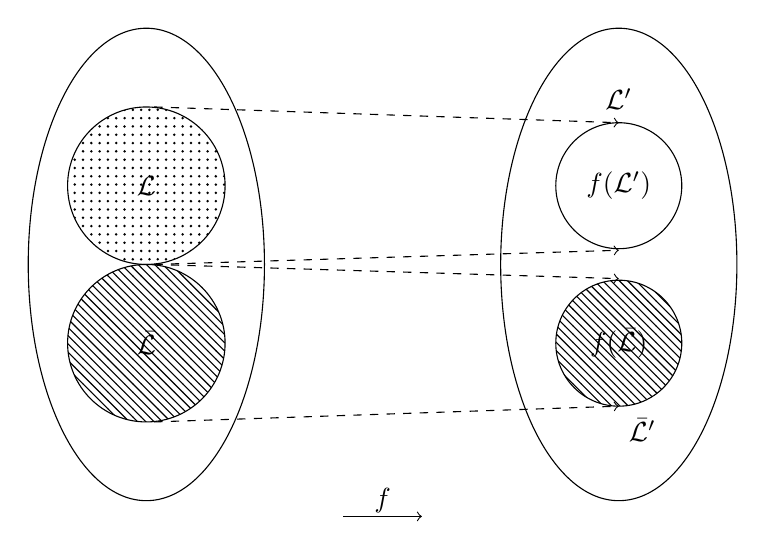
\begin{tikzpicture}

	% Left set L
	\draw (0,0) ellipse (1.5cm and 3cm);
	\draw[pattern=dots] (0,1) ellipse (1cm and 1cm);
	\draw[pattern=north west lines] (0,-1) ellipse (1cm and 1cm);

	% Right set L'
	\draw (6,0) ellipse (1.5cm and 3cm);
	\draw (6,1) ellipse (0.8cm and 0.8cm);
	\draw[pattern=north west lines] (6,-1) ellipse (0.8cm and 0.8cm);


	\node at (6,2.1) {$\mathcal{L}'$};
	\node at (6,1.0) {$f(\mathcal{L}')$};
	\node at (0.0,-1.0) {$\bar{\mathcal{L}}$};
	\node at (0.0,1.0) {${\mathcal{L}}$};

	\node at (6.3,-2.1) {$\bar{\mathcal{L}}'$};
	\node at (6.0,-1) {$f(\bar{\mathcal{L}})$};
	% Function mapping arrows
	\draw[->,dashed] (0.1,2.0) -- (6.0,1.8);
	\draw[->,dashed] (0.1,0.0) -- (6.0,0.18);
	\draw[->,dashed] (0.1,0) -- (6.0,-0.18);
	\draw[->,dashed] (0.1,-2) -- (6.0,-1.8);

	% Function label
	\node at (3,-3.0) {$f$};
	\draw[->] (2.5,-3.2) -- (3.5,-3.2);

\end{tikzpicture}
\end{document}